% !TeX root = main.tex
\documentclass{beamer}

\usepackage[utf8]{inputenc}
\usepackage{amsmath}
\usepackage{amssymb}
\usepackage{graphicx}
\usefonttheme[onlymath]{serif}
\usepackage{algorithm}
\usepackage{algpseudocode}
\usepackage{xcolor}
\setbeamertemplate{bibliography item}[text]

\AtBeginSection[]{
    \begin{frame}
        \frametitle{Outline}
        \tableofcontents[currentsection, hideothersubsections, sectionstyle=show/shaded]
    \end{frame}
}

\usetheme{Madrid}

\title{Extend L* algorithm to Learn Syntactic Monoid}
\author{Haotian Zhang}
\date{\today}

\begin{document}
    
\frame{\titlepage}



\begin{frame}
    \frametitle{Outline}
    
    \tableofcontents
\end{frame}


% --- Slide 1: Minimal DFA vs. Syntactic Monoid ---
\section{Minimal DFA vs. Syntactic Monoid}
\begin{frame}{Minimal DFA}

{\small Let $L$ be a regular language.}

\begin{block}{Minimal DFA of L, $A_L$}
    {\small The DFA with the minimum number of states that recognizes $L$.}
\begin{itemize}
    \item The set of states is the quotient set by the Myhill-Nerode (right) congruence:
    $$ w \equiv_{L} w' \iff \forall v \in \Sigma^*. (wv \in L \iff w'v \in L) $$
    The state set is $\Sigma^* / \equiv_L$.
\end{itemize}
\end{block}
\end{frame}

% --- Slide 2: Minimal DFA vs. Syntactic Monoid ---
\begin{frame}{Syntactic Monoid}

{\small Let $L$ be a regular language.}
\begin{block}{Syntactic Monoid of L, $M_L$}
The monoid with the minimum order that recognizes $L$.
\begin{itemize}
    \item The underlying set is the quotient set by the syntactic congruence:
    $$ w \cong_{L} w' \iff \forall u, v \in \Sigma^*. (uwv \in L \iff uw'v \in L) $$
    The set is $\Sigma^* / \cong_L$.
\end{itemize}
\end{block}
\end{frame}

% --- Slide 3: Example and Properties ---
\begin{frame}{Minimal DFA vs. Syntactic Monoid}

\textbf{Example:} Let $L = (ab)^* \subseteq \{a, b\}^*$.
\vspace{-0.4em} 
\begin{columns}
    \begin{column}{0.48\textwidth} % 调整宽度，留出一点空间
        \centering
        \textbf{Minimal DFA $A_L$} 
    
        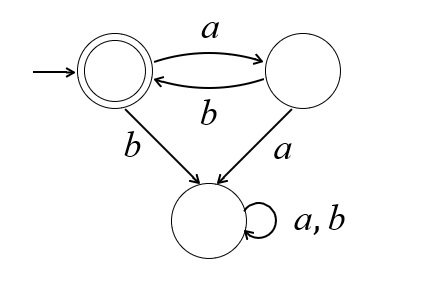
\includegraphics[width=\textwidth]{1.png} % 让图片宽度充满栏宽
        
    \end{column}

    
    \begin{column}{0.48\textwidth} % 调整宽度，留出一点空间
        \centering
        \textbf{Syntactic Monoid $M_L$} 
        
        (Right Cayley Graph) 
     
        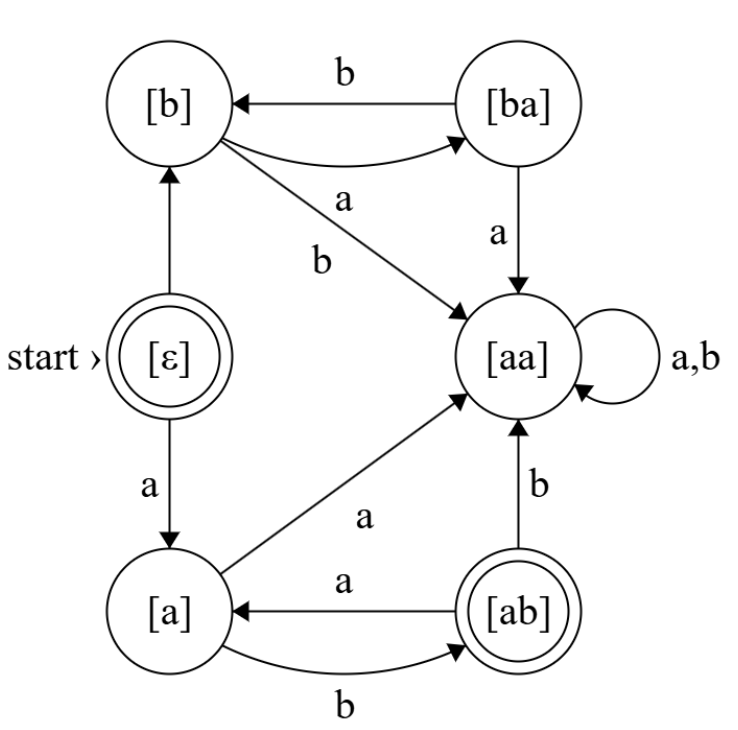
\includegraphics[width=\textwidth]{2.png} % 让图片宽度充满栏宽
    
    \end{column}
\end{columns}

\end{frame}

\begin{frame}{Properties of Syntactic Monoids}
    \begin{block}{}
        \begin{itemize}
            \item \small In general, $|M_L| \ge |A_L|$. 
            \item \small Assume $n \ge 3$ and let $A$ be an n-state deterministic finite automaton with binary input alphabet. The upper bound is $n^n - n! + g(n)$, where $g(n)$ is Landau’s
function  \cite{holzer2004deterministic}.
            \item \small Some properties can be decided more efficiently than with DFAs, e.g., star-freeness, commutativity, Green's relations, etc.
        \end{itemize}
    \end{block}


\end{frame}

% --- Slide 4: Deciding Star-Freeness ---
\section{Star-Free Language and its decision}
\begin{frame}{Star-Free Language}

\begin{definition}[Star-free Language]
{\small A language that can be expressed using concatenation of finite languages and Boolean operations ($\cup, \cap, \overline{\cdot}$).}
\end{definition}

\textbf{Example:} The language $(ab)^*$ is star-free:
$$ (ab)^* = \overline{\Sigma^*aa\Sigma^*} \cap \overline{\Sigma^*bb\Sigma^*} \cap \overline{\Sigma^*a} \cap \overline{b\Sigma^*} $$

\begin{theorem}[Schützenberger, 1965]
A regular language $L$ is star-free if and only if its syntactic monoid $M_L$ is aperiodic\cite{schutzenger65}. 
\begin{itemize}
    \item A monoid $M$ is \textbf{aperiodic} if $\forall m \in M, \exists k \in \mathbb{N} \text{ such that } m^k = m^{k+1}$.
\end{itemize}
\end{theorem}
{\small This is equivalent to its minimal DFA $A_L$ being permutation-free .}
\end{frame}

% --- Slide 5: Deciding Star-Freeness ---
\begin{frame}{Decision of Star-Freeness}
\begin{alertblock}{How to decide star-freeness?}
\begin{itemize}
    \item The determination of permutation-freeness is \textbf{ co-NP-hard} with respect to the number of states $|A_L|$ \cite{stern85}.
    \item Deciding aperiodicity is $O(n^2)$ with respect to the order $n = |M_L|$.
\end{itemize}
\end{alertblock}
\textbf{Deciding star-freeness via the syntactic monoid is considered to be efficient.}
\end{frame}

% --- Slide 6: Naive Approach to solve star-freeness judgement---
\section{L* algorithm}
\begin{frame}{L* algorithm - Learning Minimal DFA}
\begin{block}{L* algorithm -- Learning a minimal DFA}
For an unknown regular language $U \subseteq \Sigma^*$, find $U$'s expression using two types of queries:\cite{angluin87}
\begin{itemize}
    \item \textbf{Membership query:} For a word $w \in \Sigma^*$, is $w \in U$?
    \item \textbf{Equivalence query:} For a DFA $\mathcal{A}$, is $L(\mathcal{A}) = U$? If the answer is no, then we can obtain a counterexample. 
\end{itemize}
\end{block}



\end{frame}
% --- Slide 7: L* algorithm ---
\begin{frame}{L* algorithm - Observation Table }
\begin{columns}[T]

    % --- 左栏：修改后，宽度变小，内容更紧凑 ---
    \begin{column}{0.6\textwidth}
        \begin{itemize}
            \item $U$ : Unknown regular language
            \item $\Sigma$ : Alphabet, in example it is $\{a,b\}$
            \item $I$ : Set of test states
            \item $S$ : Set of suffixes
            \item $T$: $(I \cup I \cdot \Sigma \times S) \to \{0,1\}$
            \item $OT$ : {\small Observation table. Actually it is a 3-tuple } $(I,S,T)$
            \item $status$: A function $status:= S \rightarrow\{0,1\}$. And $status_i(s) = T(i,s)$
        \end{itemize}
    \end{column}

    % --- 右栏：修正后，宽度变大，表格格式正确 ---
    \begin{column}{0.6\textwidth}
        \centering
        \begin{tabular}{cc|c|c}
            &   & \multicolumn{2}{c}{$S$} \\ % 表头是 S (Suffixes)
            \multicolumn{2}{c|}{} & $\epsilon$ & a \\ \hline
            & $\epsilon$ & 1 & 0 \\
            {$I$}& a          & 0 & 1 \\
            & b          & 0 & 0 \\\hline
            
            & aa& 1& 0 \\
{$I\cdot \Sigma$}        & ab& 0&0\\
            & ba         & 0 & 0 \\
            & bb         & 1 & 0 \\ 
           
            
        \end{tabular}
    \end{column}
    
\end{columns}
\end{frame}


% --- Slide 8: L* algorithm ---
\begin{frame}{L* algorithm - Closed \&  Separable}
\textbf{Suffix-equivalent for $u, v \in \Sigma^{*}$: }
$$
    i \equiv_{S} i^{\prime} \Leftrightarrow  \forall s \in S .status_i(s) = status_{i^{\prime}}(s)
$$
\textbf{\small Separable}: \small no two distinct words in $I$ are \textbf{Suffix-equivalent}. 


\textbf{Closed: }
$$
    \forall w \in I , a \in \Sigma, \exists w^{\prime} \in I.wa \equiv_{S} w
$$
        \centering
        \begin{tabular}{cc|c|c}
            &   & \multicolumn{2}{c}{$S$} \\ % 表头是 S (Suffixes)
            \multicolumn{2}{c|}{} & $\epsilon$ & a \\ \hline
            & $\epsilon$ & 1 & 0 \\
            {$I$}& a          & 0 & 1 \\
            & b          & 0 & 0 \\ \hline
            
            & aa& 1& 0 \\
{$I \cdot \Sigma$}& ab& 0&0\\
            & ba         & 0 & 0 \\
            & bb         & 1 & 0 \\  
        \end{tabular}
\end{frame}

% --- Slide 9: L* algorithm ---
\begin{frame}{L* algorithm - Algorithmic Process}
1. $I:= S := \{\epsilon\}$\\
2. If $OT$ is not closed but separable, use \textbf{membership queries} to find a $w^{\prime} \in I \cdot \Sigma$, which for any $s\in S$ , $status_{w^{\prime}}(s)$ is different from any $status_{w}(s),w \in I$. Add $w^{\prime}$ to $I$ and expand $I \cdot \Sigma$. Repeat this operation until $OT$ is separable and closed.\\
3. We can get an \textbf{Acceptor} (hypothesis automaton) and ask an \textbf{equivalence query} for it. \\
4. If the answer is yes, algorithm terminates and \textbf{Acceptor} is the answer. \\
5. If the answer is no, find a counterexample $w$ in $O(log|w|)$\cite{Worrell:DFALearning}. Properly expand $I$ and $S$. Now $OT$ must not be closed. \\
6. Return to 2.
\end{frame}
% --- Slide 10: Aspects of deciding star-freeness ---
\begin{frame}{Aspects of deciding star-freeness}
\begin{block}{Naive Approach (Inefficient)}
Use Angluin's L*-algorithm to construct the minimal DFA $A_L$, and then:
\begin{enumerate}
    \item Decide if $A_L$ is permutation-free (\textbf{co-NP-hard}).
    \item Convert $A_L$ to the syntactic monoid $M_L$ and check for aperiodicity (the conversion can cause an \textbf{explosion in the number of states}).
\end{enumerate}
\end{block}

\begin{center}
    \textbf{\small Goal: We want to construct the syntactic monoid $M_L$ directly!}
\end{center}
    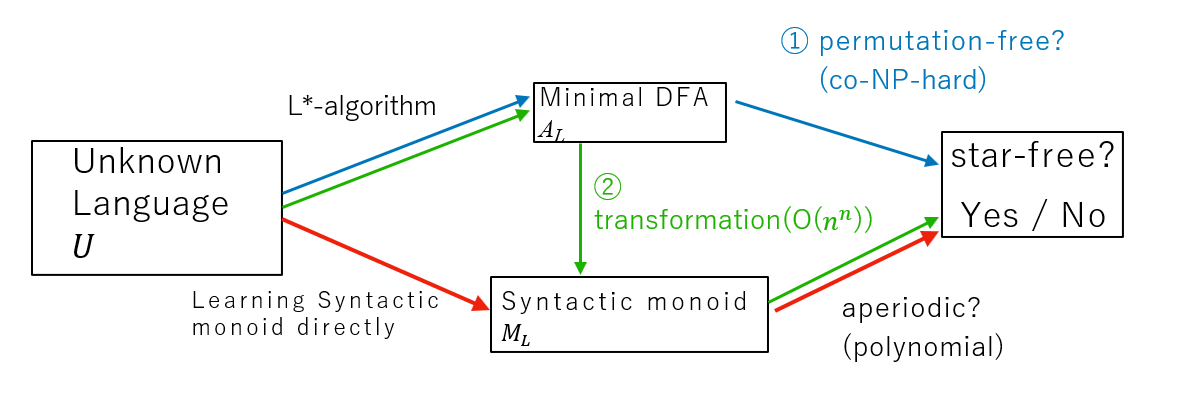
\includegraphics[width=0.9\textwidth]{3.png}
\end{frame}

% --- Slide 11: Learning Syntactic Monoid ---
\section{Idea of Learning Syntactic Monoid}
\begin{frame}{Idea - Learning Syntactic Monoid}
    \begin{itemize}
            \item $U$ : Unknown regular language
            \item $\Sigma$ : Alphabet
            \item \textbf{\color{red}{$P$}} : Set of prefixes
            \item $S$ : Set of suffixes
            \item $I$ : Set of test states
            \item \textbf{\color{red}{$T$}}: $P\times (I \cup I \cdot \Sigma) \times S \to \{0,1\}$
            \item \textbf{\color{red}{$OT$}} : {\small Observation table. Actually it is a 4-tuple} $(P,I,S,T)$
            \item \textbf{\color{red}{$status$}}: A function $status:= (P \times S) \rightarrow\{0,1\}$. And $status_i (p,s) = T(p,i,s)$
    \end{itemize}    
\end{frame}


% --- Slide 12: Learning Syntactic Monoid ---
\begin{frame}{Idea - Closed \& Separable}
\textbf{Status-equivalent for $i, i^{\prime}\in \Sigma^{*}$: }
$$
    i \equiv_{status} i^{\prime} \Leftrightarrow  \forall p \in P,s \in S. status_i(p,s) = status_{i^{\prime}}(p,s)
$$
\textbf{Separable}: no two distinct words in $I$ are \textbf{Status-equivalent}. 


\textbf{Closed: }
$$
    \forall i^{\prime} \in I\cdot \Sigma ,  \exists i \in I.(i \equiv_{status} i^{\prime})
$$


\end{frame}
% --- Slide 13: Learning Syntactic Monoid ---
\begin{frame}{Idea -- Process}
1. $I := \{\epsilon\}$, $P:=S:= \{\epsilon\} \cup \Sigma$

2. If $OT$ is not closed but separable, use \textbf{membership queries} to find an $i \in I \cdot \Sigma$, which $status_i$ is different from any $status_{i^{\prime}}, i^{\prime}\in I$. Add $i$ to $I$ and expand $I \cdot \Sigma$.

Repeat this operation until $OT$ is separable and closed.

3. We can get an \textbf{Acceptor} (hypothesis automaton) and ask an \textbf{equivalence query} for it. 

4. If the answer is yes, algorithm terminates and \textbf{Acceptor} is the answer. 

5. If the answer is no, find a counterexample. Properly expand $I$, $P$ and $S$. Then $OT$ must not be closed. 

6. Return to 2.

\end{frame}


% --- Slide 15: Learning Syntactic Monoid ---
\begin{frame}{Idea -- Example}
$$
L = \Sigma \cdot \Sigma \cdot \Sigma \cdot b^* + \Sigma \cdot \Sigma \cdot  \Sigma +\Sigma \cdot \Sigma+ \Sigma + \epsilon\ 
$$
 
   
        \centering
        \resizebox{\columnwidth}{!}{% % \columnwidth 是当前列的宽度 (0.5\textwidth)
        \begin{tabular}{|cc|*{9}{c|}}
            \multicolumn{2}{c|}{} & \multicolumn{9}{c}{$(P\times S)$}\\
            \multicolumn{2}{c|}{} & $(\epsilon,\epsilon)$& $(\epsilon,a)$& $(\epsilon,b)$&$(a,\epsilon)$&$(a,a)$& $(a,b)$&$(b,\epsilon)$ & $(b,a)$&$(b,b)$\\ \hline
            $I$ & $\epsilon$ & 1 & 1& 1& 1& 1& 1& 1& 1&1\\\hline
            $I \cdot \Sigma$ & a& 1& 1& 1& 1& 1& 1& 1& 1&1\\
            & b& 1&1& 1& 1& 1& 1& 1& 1&1\\
        \end{tabular}
        }

Counterexample : $aaaa$.
\end{frame}


% --- Slide 16: Learning Syntactic Monoid ---
\begin{frame}{Idea -- Example}
    % --- 第一个表格 ---
    \centering  % 让表格居中
    \resizebox{\linewidth}{!}{%
        \begin{tabular}{|cc|*{9}{c|}}
            \multicolumn{2}{c|}{} & \multicolumn{9}{c}{$(P\times S)$}\\
            \multicolumn{2}{c|}{} & $(\epsilon,\epsilon)$& $(\epsilon,a)$& $(\epsilon,b)$&$(\epsilon,aa)$&$(\epsilon,aaa)$& $(\epsilon,aaaa)$&$(a,\epsilon)$& $(a,a)$&$(a,b)$\\ \hline
            $I$ & $\epsilon$ & 1 & 1& 1& 1& 1& 0& 1& 1&1\\\hline
            $I \cdot \Sigma$ & a& 1& 1& 1& 1& 0& 0& 1& 1&1\\
            & b& 1&1& 1& 1& 0& 0& 1& 1&1\\
        \end{tabular}
    }

    % --- 垂直间距 ---
    \vspace{1em} % 在两个表格之间增加一点空隙，可以改为 0.5cm 或 \vfill

    % --- 第二个表格 ---
    \resizebox{\linewidth}{!}{%
        \begin{tabular}{cc|c|c|c|c|c|c|c|c|c|}
            &   & \multicolumn{9}{c}{$(P\times S)$}\\ 
            \multicolumn{2}{c|}{} & $(a,aa)$& $(a,aaa)$& $(a,aaaa)$&$(b,\epsilon)$&$(b,a)$& $(b,b)$&$(b,aa)$& $(b,aaa)$&$(b,aaaa)$\\ \hline
            {$I$}& $\epsilon$ & 1 & 0& 0& 1& 1& 1& 1& 0&0\\\hline
            & a& 0& 0& 0& 1& 1& 1& 0& 0&0\\
            {$I \cdot \Sigma$}& b& 0&0& 0& 1& 1& 1& 0& 0&0\\  
        \end{tabular}
    }
    
    \vspace{0.5em}
    \raggedright % 如果想让最后的文字靠左，加上这个；如果不加，因为上面写了 \centering，这句话也会居中
    Some parts are omitted. 
\end{frame}


% --- Slide 17: Learning Syntactic Monoid ---
\begin{frame}{Idea -- Example}

        \centering
        \resizebox{\linewidth}{!}{
        \begin{tabular}{cc|c|c|c|c|c|c|c|c|c|}
            &   & \multicolumn{9}{c}{$(P\times S)$}\\ % 表头是 S (Suffixes)
            \multicolumn{2}{c|}{} & $(\epsilon,\epsilon)$& $(\epsilon,a)$& $(\epsilon,b)$&$(\epsilon,aa)$&$(\epsilon,aaa)$& $(\epsilon,aaaa)$&$(a,\epsilon)$& $(a,a)$&$(a,b)$\\ \hline
            {$I$}& $\epsilon$ & 1 & 1& 1& 1& 1& 0& 1& 1&1\\
            
            & $a$& 1& 1& 1& 1& 0& 0& 1& 1&1\\ \hline
            
& $b \equiv_{status} a$& 1&1& 1& 1& 0& 0& 1& 1&1\\
 {$I \cdot \Sigma$}& $aa$& 1& 1& 1& 0& 0& 0& 1& 0&1\\
 & $ab$& 1& 1& 1& 0& 0& 0& 1& 0&1\\  
        \end{tabular}
        }

    \vspace{1em} % 在两个表格之间增加一点空隙，可以改为 0.5cm 或 \vfill
        \resizebox{\linewidth}{!}{
        \begin{tabular}{cc|c|c|c|c|c|c|c|c|c|}
            &   & \multicolumn{9}{c}{$(P\times S)$}\\ % 表头是 S (Suffixes)
            \multicolumn{2}{c|}{} & $(a,aa)$& $(a,aaa)$& $(a,aaaa)$&$(b,\epsilon)$&$(b,a)$& $(b,b)$&$(b,aa)$& $(b,aaa)$&$(b,aaaa)$\\ \hline
            {$I$}& $\epsilon$ & 1 & 0& 0& 1& 1& 1& 1& 0&0\\
            
            & $a$& 0& 0& 0& 1& 1& 1& 0& 0&0\\ \hline
& $b \equiv_{status} a$& 0&0& 0& 1& 1& 1& 0& 0&0\\
 {$I \cdot \Sigma$}& $aa$& 0& 0& 0& 1& 0& 1& 0& 0&0\\
 & $ab$& 0& 0& 0& 1& 0& 1& 0& 0&0\\  
        \end{tabular}
        }
    \end{frame}

% --- Slide 18: Learning Syntactic Monoid ---
\begin{frame}{Idea -- Example}
 
        \centering
        \resizebox{\linewidth}{!}{
        \begin{tabular}{cc|c|c|c|c|c|c|c|c|c|}
            &   & \multicolumn{9}{c}{$(P\times S)$}\\ % 表头是 S (Suffixes)
            \multicolumn{2}{c|}{} & $(\epsilon,\epsilon)$& $(\epsilon,a)$& $(\epsilon,b)$&$(\epsilon,aa)$&$(\epsilon,aaa)$& $(\epsilon,aaaa)$&$(a,\epsilon)$& $(a,a)$&$(a,b)$\\ \hline
            & $\epsilon$ & 1 & 1& 1& 1& 1& 0& 1& 1&1\\
            
            {$I$}& $a$& 1& 1& 1& 1& 0& 0& 1& 1&1\\
 & $aa$& 1& 1& 1& 0& 0& 0& 1& 0&1\\ \hline
            
& $b \equiv_{status} a$& 1&1& 1& 1& 0& 0& 1& 1&1\\
 {$I \cdot \Sigma$}& $ab \equiv_{status} aa$& 1& 1& 1& 0& 0& 0& 1& 0&1\\
 & $aaa$& 1& 0& 1& 0& 0& 0& 0& 0&0\\
 & $aab$& 1& 0& 1& 0& 0& 0& 1& 0&1\\  
        \end{tabular}
        }
    \vspace{1em} % 在两个表格之间增加一点空隙，可以改为 0.5cm 或 \vfill
        \centering
        \resizebox{\linewidth}{!}{
        \begin{tabular}{cc|c|c|c|c|c|c|c|c|c|}
            &   & \multicolumn{9}{c}{$(P\times S)$}\\ % 表头是 S (Suffixes)
            \multicolumn{2}{c|}{} & $(a,aa)$& $(a,aaa)$& $(a,aaaa)$&$(b,\epsilon)$&$(b,a)$& $(b,b)$&$(b,aa)$& $(b,aaa)$&$(b,aaaa)$\\ \hline
            & $\epsilon$ & 1 & 0& 0& 1& 1& 1& 1& 0&0\\
            
            {$I$}& $a$& 0& 0& 0& 1& 1& 1& 0& 0&0\\
 & $aa$& 0& 0& 0& 1& 0& 1& 0& 0&0\\ \hline
& $b \equiv_{status} a$& 0&0& 0& 1& 1& 1& 0& 0&0\\
 {$I \cdot \Sigma$}& $ab \equiv_{status} aa$& 0& 0& 0& 1& 0& 1& 0& 0&0\\
 & $aaa$& 0& 0& 0& 0& 0& 0& 0& 0&0\\
 & $aab$& 0& 0& 0& 1& 0& 1& 0& 0&0\\  
        \end{tabular}
        }
    \end{frame}

    % --- Slide 19: Learning Syntactic Monoid ---
\begin{frame}{Idea -- Example}
        \centering
        \resizebox{\linewidth}{!}{
        \begin{tabular}{cc|c|c|c|c|c|c|c|c|c|}
            &   & \multicolumn{9}{c}{$(P\times S)$}\\ % 表头是 S (Suffixes)
            \multicolumn{2}{c|}{} & $(\epsilon,\epsilon)$& $(\epsilon,a)$& $(\epsilon,b)$&$(\epsilon,aa)$&$(\epsilon,aaa)$& $(\epsilon,aaaa)$&$(a,\epsilon)$& $(a,a)$&$(a,b)$\\ \hline
            & $\epsilon$ & 1 & 1& 1& 1& 1& 0& 1& 1&1\\
            
            {$I$}& $a$& 1& 1& 1& 1& 0& 0& 1& 1&1\\
 & $aa$& 1& 1& 1& 0& 0& 0& 1& 0&1\\
 & $aaa$& 1& 0& 1& 0& 0& 0& 0& 0&0\\ \hline
            
& $b \equiv_{status} a$& 1&1& 1& 1& 0& 0& 1& 1&1\\
 & $ab \equiv_{status} aa$& 1& 1& 1& 0& 0& 0& 1& 0&1\\
 {$I \cdot \Sigma$}& $aab$& 1& 0& 1& 0& 0& 0& 1& 0&1\\
 & $aaaa$& 0& 0& 0& 0& 0& 0& 0& 0&0\\
 & $aaab$& 1& 0& 1& 0& 0& 0& 0& 0&0\\  
        \end{tabular}
        }
    \vspace{1em} % 在两个表格之间增加一点空隙，可以改为 0.5cm 或 \vfill
        \centering
        \resizebox{\linewidth}{!}{
        \begin{tabular}{cc|c|c|c|c|c|c|c|c|c|}
            &   & \multicolumn{9}{c}{$(P\times S)$}\\ % 表头是 S (Suffixes)
            \multicolumn{2}{c|}{} & $(a,aa)$& $(a,aaa)$& $(a,aaaa)$&$(b,\epsilon)$&$(b,a)$& $(b,b)$&$(b,aa)$& $(b,aaa)$&$(b,aaaa)$\\ \hline
            & $\epsilon$ & 1 & 0& 0& 1& 1& 1& 1& 0&0\\
            
            {$I$}& $a$& 0& 0& 0& 1& 1& 1& 0& 0&0\\
 & $aa$& 0& 0& 0& 1& 0& 1& 0& 0&0\\
 & $aaa$& 0& 0& 0& 0& 0& 0& 0& 0&0\\ \hline
& $b \equiv_{status} a$& 0&0& 0& 1& 1& 1& 0& 0&0\\
 & $ab \equiv_{status} aa$& 0& 0& 0& 1& 0& 1& 0& 0&0\\
 {$I \cdot \Sigma$}& $aab$& 0& 0& 0& 1& 0& 1& 0& 0&0\\
 & $aaaa$& 0& 0& 0& 0& 0& 0& 0& 0&0\\
 & $aaab\equiv_{status} aaa$& 0& 0& 0& 0& 0& 0& 0& 0&0\\  
        \end{tabular}
        }
    \end{frame}


   % --- Slide 20: Learning Syntactic Monoid ---
\begin{frame}{Idea -- Example}

        \centering
        \resizebox{\linewidth}{!}{
        \begin{tabular}{cc|c|c|c|c|c|c|c|c|c|}
            &   & \multicolumn{9}{c}{$(P\times S)$}\\ % 表头是 S (Suffixes)
            \multicolumn{2}{c|}{} & $(\epsilon,\epsilon)$& $(\epsilon,a)$& $(\epsilon,b)$&$(\epsilon,aa)$&$(\epsilon,aaa)$& $(\epsilon,aaaa)$&$(a,\epsilon)$& $(a,a)$&$(a,b)$\\ \hline
            & & & & & & & & & &\\
            
            {$I$}& $\cdots$& & & & & & & & &\\
 & $aab$& 1& 0& 1& 0& 0& 0& 1& 0&1\\ \hline
            
& $b \equiv_{status} a$& 1&1& 1& 1& 0& 0& 1& 1&1\\
 & $ab \equiv_{status} aa$& 1& 1& 1& 0& 0& 0& 1& 0&1\\
 {$I \cdot \Sigma$}& $aaaa$& 0& 0& 0& 0& 0& 0& 0& 0&0\\
 & $aaab\equiv_{status} aaa$& 1& 0& 1& 0& 0& 0& 0& 0&0\\
 & $aaba$& 0& 0& 0& 0& 0& 0& 0& 0&0\\
 & $aabb \equiv_{status} aab$& 1& 0& 1& 0& 0& 0& 1& 0&1\\  
        \end{tabular}
        }

        \resizebox{\linewidth}{!}{
        \begin{tabular}{cc|c|c|c|c|c|c|c|c|c|}
            &   & \multicolumn{9}{c}{$(P\times S)$}\\ % 表头是 S (Suffixes)
            \multicolumn{2}{c|}{} & $(a,aa)$& $(a,aaa)$& $(a,aaaa)$&$(b,\epsilon)$&$(b,a)$& $(b,b)$&$(b,aa)$& $(b,aaa)$&$(b,aaaa)$\\ \hline
            & & & & & & & & & &\\
            
            {$I$}& $\cdots$& & & & & & & & &\\
 & $aab$& 0& 0& 0& 1& 0& 1& 0& 0&0\\ \hline
& $b \equiv_{status} a$& 0&0& 0& 1& 1& 1& 0& 0&0\\
 & $ab \equiv_{status} aa$& 0& 0& 0& 1& 0& 1& 0& 0&0\\
 {$I \cdot \Sigma$}& $aaaa$& 0& 0& 0& 0& 0& 0& 0& 0&0\\
 & $aaab\equiv_{status} aaa$& 0& 0& 0& 0& 0& 0& 0& 0&0\\
 & $aaba$& 0& 0& 0& 0& 0& 0& 0& 0&0\\
 & $aabb \equiv_{status} aab$& 0& 0& 0& 1& 0& 1& 0& 0&0\\  
        \end{tabular}
        }
    \end{frame}


   % --- Slide 21: Learning Syntactic Monoid ---
\begin{frame}{Idea -- Example}
 
        \centering
        \resizebox{\linewidth}{!}{
        \begin{tabular}{cc|c|c|c|c|c|c|c|c|c|}
            &   & \multicolumn{9}{c}{$(P\times S)$}\\ % 表头是 S (Suffixes)
            \multicolumn{2}{c|}{} & $(\epsilon,\epsilon)$& $(\epsilon,a)$& $(\epsilon,b)$&$(\epsilon,aa)$&$(\epsilon,aaa)$& $(\epsilon,aaaa)$&$(a,\epsilon)$& $(a,a)$&$(a,b)$\\ \hline
            & & & & & & & & & &\\
            
            {$I$}& $\cdots$& & & & & & & & &\\
 & $aaaa$& 0& 0& 0& 0& 0& 0& 0& 0&0\\ \hline
            
& $b \equiv_{status} a$& 1&1& 1& 1& 0& 0& 1& 1&1\\
 & $ab \equiv_{status} aa$& 1& 1& 1& 0& 0& 0& 1& 0&1\\
 {$I \cdot \Sigma$}& $aaab\equiv_{status} aaa$& 1& 0& 1& 0& 0& 0& 0& 0&0\\
 & $aaba$& 0& 0& 0& 0& 0& 0& 0& 0&0\\
 & $aabb \equiv_{status} aab$& 1& 0& 1& 0& 0& 0& 1& 0&1\\
 & $aaaaa$& 0& 0& 0& 0& 0& 0& 0& 0&0\\
 & $aaaab$& 0& 0& 0& 0& 0& 0& 0& 0&0\\  
        \end{tabular}
        }
    \vspace{1em} % 在两个表格之间增加一点空隙，可以改为 0.5cm 或 \vfill
        \resizebox{\linewidth}{!}{
        \begin{tabular}{cc|c|c|c|c|c|c|c|c|c|}
            &   & \multicolumn{9}{c}{$(P\times S)$}\\ % 表头是 S (Suffixes)
            \multicolumn{2}{c|}{} & $(a,aa)$& $(a,aaa)$& $(a,aaaa)$&$(b,\epsilon)$&$(b,a)$& $(b,b)$&$(b,aa)$& $(b,aaa)$&$(b,aaaa)$\\ \hline
            & & & & & & & & & &\\
            
            {$I$}& $\cdots$& & & & & & & & &\\
 & $aaaa$& 0& 0& 0& 0& 0& 0& 0& 0&0\\ \hline
& $b \equiv_{status} a$& 0&0& 0& 1& 1& 1& 0& 0&0\\
 & $ab \equiv_{status} aa$& 0& 0& 0& 1& 0& 1& 0& 0&0\\
 {$I \cdot \Sigma$}& $aaab\equiv_{status} aaa$& 0& 0& 0& 0& 0& 0& 0& 0&0\\
 & $aaba$& 0& 0& 0& 0& 0& 0& 0& 0&0\\
 & $aabb \equiv_{status} aab$& 0& 0& 0& 1& 0& 1& 0& 0&0\\
 & $aaaaa$& 0& 0& 0& 0& 0& 0& 0& 0&0
\\
 & $aaaab$& 0& 0& 0& 0& 0& 0& 0& 0&0\\  
        \end{tabular}
        }
    \end{frame}

      % --- Slide 22: Learning Syntactic Monoid ---
\begin{frame}{Idea -- Example}
        \centering
        \resizebox{\linewidth}{!}{
        \begin{tabular}{cc|c|c|c|c|c|c|c|c|c|}
            &   & \multicolumn{9}{c}{$(P\times S)$}\\ % 表头是 S (Suffixes)
            \multicolumn{2}{c|}{} & $(\epsilon,\epsilon)$& $(\epsilon,a)$& $(\epsilon,b)$&$(\epsilon,aa)$&$(\epsilon,aaa)$& $(\epsilon,aaaa)$&$(a,\epsilon)$& $(a,a)$&$\cdots$\\ \hline
            & $\epsilon$ & 1 & 1& 1& 1& 1& 0& 1& 1&\\
 & $a$& 1& 1& 1& 1& 0& 0& 1& 1&\\
 & $aa$& 1& 1& 1& 0& 0& 0& 1& 0&\\
            
            {$I$}& $aaa$& 1& 0& 1& 0& 0& 0& 0& 0&\\
 & $aab$& 1& 0& 1& 0& 0& 0& 1& 0&\\
 & $aaaa$& 0& 0& 0& 0& 0& 0& 0& 0&\\  
        \end{tabular}
        }
    $$
        I\cdot \Sigma = \{b,ab,aaab,aaba,aabb,aaaaa,aaaab\}
    $$
    $b \equiv_{status} a$, $ab \equiv_{status} aa$, $aaab\equiv_{status} aaa$, $aabb \equiv_{status} aab$
\end{frame}

% --- Slide : Progress ---
\section{Future work}
\begin{frame}{Progress}

\begin{block}{Summary}
    Modifying the observation table to check both prefixes and suffixes, because of the definition of syntactic congruence.
\end{block}

\begin{block}{Challenges}
    \begin{itemize}
        \item How to deal with the counterexample? : Now we just add all its suffixes into $S$ and all its prefixes into $P$. Is there a better way to handle it?
        \item Proof of correctness.
    \end{itemize}
\end{block}

\end{frame}

% --- Slide : Future work ---
\begin{frame}{Future work}

\begin{block}{Computational cost and Improvement}
To theoretically evaluate if the extension algorithm is a polynomial-time algorithm for learning the syntactic monoid $M_L$ from an unknown regular language $L$.

Reduce useless information during the process to improve computational cost. 
\end{block}

\begin{block}{Evaluation}
     Using this approach, implement the algorithm and evaluate its efficiency and usability for problems such as the \textbf{decidability of star-free languages}.
\end{block}
\end{frame}

% --- Slide 16:  --- 
\begin{frame}[allowframebreaks] % allowframebreaks 选项允许参考文献列表自动分页
\frametitle{References}

% 设置参考文献的样式
\bibliographystyle{IEEEtran} % plain, alpha, unsrt 等样式都可以

% 指定你的 .bib 文件
% myrefs 是你的 .bib 文件的名字 (不带 .bib 后缀)
\bibliography{reference} 

\end{frame}

\end{document}